\chapter{Demonstration Problems} 
\label{demos}

Radiation transport and mobile depletion play an important role in many areas of health physics and environmental impact modelling. A critical application of these methods is to analyze ex-core neutron fields for the purposes of work planning and radiation dose mitigation in containment systems. Ex-core neutron fields also prove useful in determining the concentration fields of radioactive effluents, allowing for the prediction of operational releases of radioactive material. A second use for these methods is to determine the photon fluxes emitted from a plume of radioactive material in the event of a release from a nuclear reactor or release from a containment system. Though the goal of this work was to develop the capabilities to perform analyses of these types within \texttt{Caribou}, the tool was used to perform several calculations that demonstrate its capabilities. The first of these demonstration problems is the formation of the radionuclide effluent $\mathrm{^{41}Ar}$ in a small \acrfull{bwr} containment structure. The second demonstration problem showcases the coupled solvers being used to predict the transport of a $\mathrm{^{137}Cs}$ plume out of a containment structure and the associated photon flux from the decay of $\mathrm{^{137m}Ba}$.

\section{Ar-41 Formation in a Small BWR Structure}
\label{demos:demonstrations:ar41_bwr}

The first demonstration problem evaluates the formation of $\mathrm{^{41}Ar}$ in a 2D model of a small \acrshort{bwr} containment system. $\mathrm{^{41}Ar}$ forms in a neutron field through the following reaction with  $\mathrm{^{40}Ar}$ in air:
\begin{equation*}
    \mathrm{^{40}Ar}\, \xrightarrow{\mathrm{(n,\gamma)}} \,\mathrm{^{41}Ar}\text{.}
\end{equation*}

\begin{figure}[H]
    \centering
    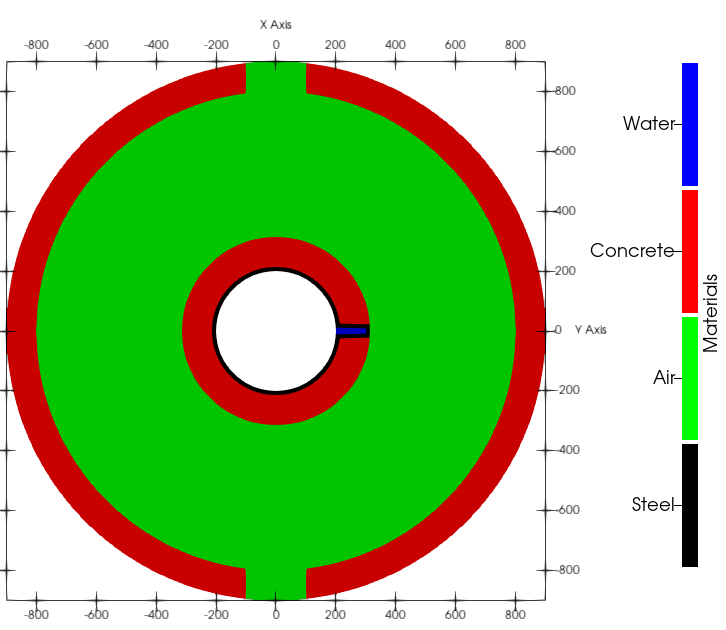
\includegraphics[width=0.725\textwidth]{images/demos/bwr_shield/geo.png}
    \caption{2D representative containment system for a small \acrshort{bwr}. All units are in cm.}
    \label{fig:demo:bwr:geo:cont_full}
\end{figure}

This system consists of a light water spectrum reactor with an effective core radius of 200 cm. This reactor is surrounded by a steel reactor pressure vessel with a thickness of 14 cm. The reactor is encased in a 100 cm thick biological shield made of concrete. This biological shield is penetrated by a pipe from the heat transport system, which is 22 cm wide, 100 cm long, and has a wall thickness of 14 cm. The pipe itself is made of steel and is filled with light water. The containment walls are separated from the biological shield by approximately 486 cm and are 100 cm thick. Finally, the containment structure has two airlocks each of which are 200 cm wide. A representation of the geometry of this demonstration problem can be found in Figure~\ref{fig:demo:bwr:geo:cont_full}.

\begin{figure}[H]
    \centering
    \begin{subfigure}[b]{0.495\textwidth}
        \centering
        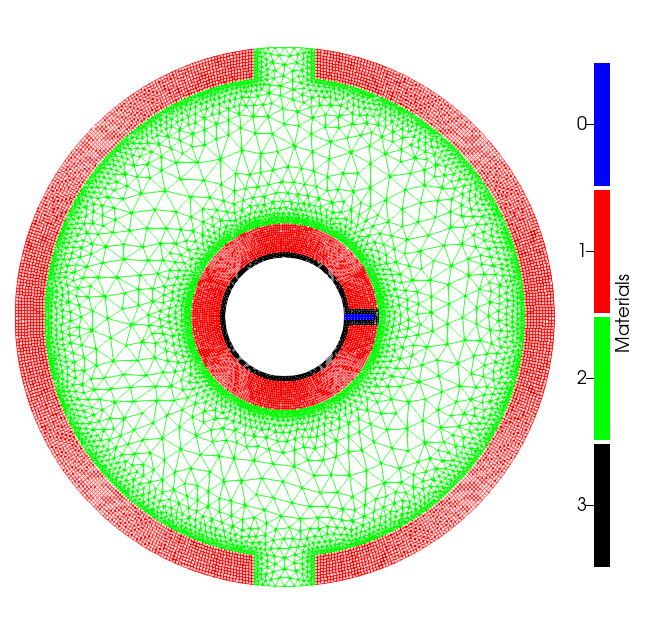
\includegraphics[width=\textwidth]{images/demos/bwr_shield/neu_mesh.png}
        \caption{Full mesh.}
        \label{fig:demo:bwr:mesh:neu_full}
    \end{subfigure}
    \hfill
    \begin{subfigure}[b]{0.495\textwidth}
        \centering
        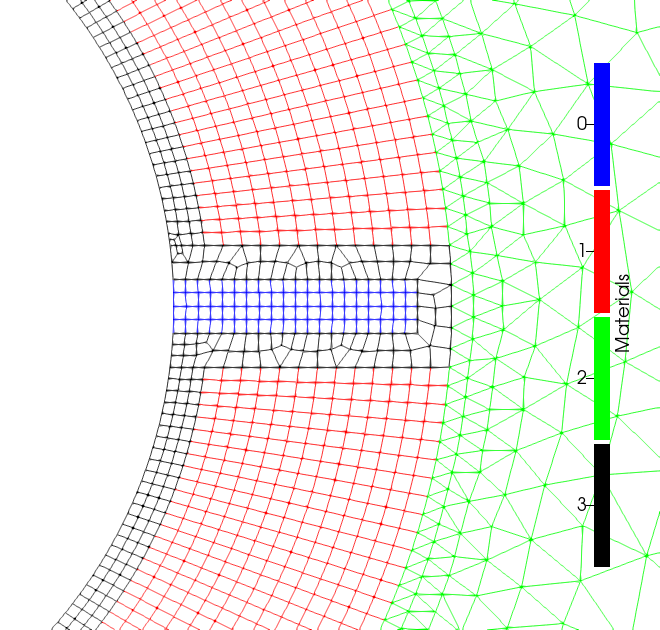
\includegraphics[width=\textwidth]{images/demos/bwr_shield/neu_mesh_close.png}
        \caption{Mesh refinement near the penetration in the biological shield.}
        \label{fig:demo:bwr:mesh:neu_streaming}
    \end{subfigure}
    \caption{Mesh used for the 2D neutron transport calculations in a containment system.}
    \label{fig:demo:bwr:neu_mesh}
\end{figure}

The modelling of the neutron fields in this containment system was performed with the developed \acrshort{sn} radiation transport solver without ray effect mitigation measures. In lieu of simulating a full \acrshort{bwr} in the center of the containment system, a uniform current boundary condition was applied to the inner face of the reactor pressure vessel with a spectrum assumed to be that of a $\mathrm{^{252}Cf}$ neutron source moderated by $\mathrm{D_{2}O}$ \cite{iso_neutron}. This was done to avoid the statistical penalty imposed on the surface source and cross sections caused by the addition of a \acrshort{bwr} to the \texttt{OpenMC} model and is considered sufficient for the proof of principle calculations performed in this work; production calculations should use surface sources computed from reactor models. The remaining boundaries along the outer walls of the containment structure and airlocks are vacuum boundary conditions. Transport corrected neutron cross sections and the associated net current were calculated using \texttt{OpenMC} \cite{openmc} with the CASMO-8 group structure. The problem was meshed with Coreform Cubit using a mixture of triangular and quadrilateral elements with a total element count of 15,390. Care was taken to ensure that the element density was high in the concrete, biological shield, and streaming penetration due to the rapid variation of the scalar fluxes in different energy groups due to down-scattering and absorption. The mesh used for the radiation transport calculation can be found in Figure~\ref{fig:demo:bwr:mesh:neu_full} with a separate view showing the element density for the streaming penetration in Figure~\ref{fig:demo:bwr:mesh:neu_streaming}.

The neutron transport simulation used a Gauss-Chebyshev product quadrature with 5 polar angles and 5 azimuthal angles, resulting in a total of 100 angular unknowns per energy group as there are four octants of the unit sphere in 2D calculations. This case used the \acrshort{pjfnk} solver with preconditioning provided by the hypre package BoomerAMG and 10 \acrshort{gmres} vectors. A relative convergence criteria of $10^{-8}$ was used based on the initial residual vector magnitude of $9.82696\times 10^{-1}$. A sample of the resulting neutron fields in the containment system can be found in Figure~\ref{fig:demo:bwr:neutron}.

\begin{figure}[H]
    \centering
    \begin{subfigure}[b]{0.495\textwidth}
        \centering
        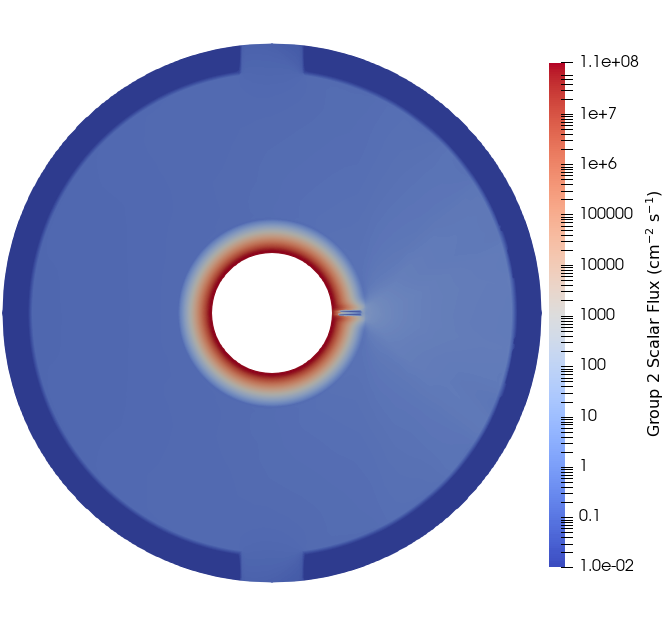
\includegraphics[width=\textwidth]{images/demos/bwr_shield/neutron_field/group_2.png}
        \caption{Group 2 neutron flux ($5.53\times 10^{3}\text{ eV } \leq E < 8.21\times 10^{5}\text{ eV}$).}
        \label{fig:demo:bwr:neutron:g2}
    \end{subfigure}
    \hfill
    \begin{subfigure}[b]{0.495\textwidth}
        \centering
        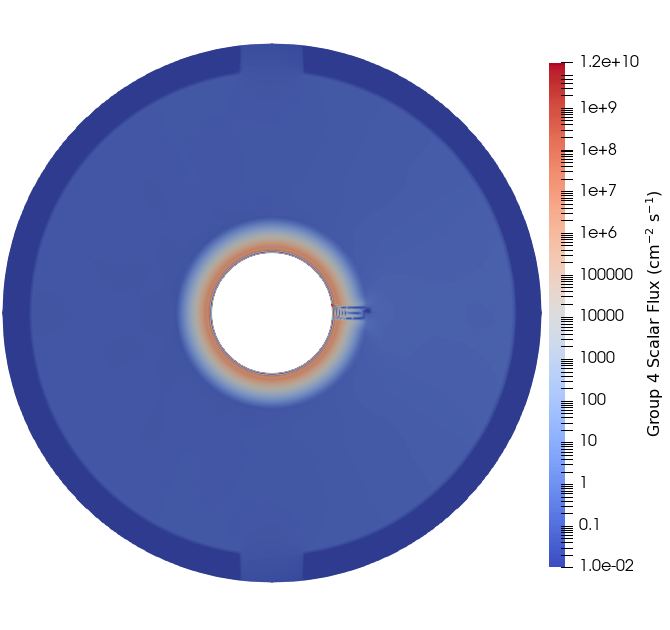
\includegraphics[width=\textwidth]{images/demos/bwr_shield/neutron_field/group_4.png}
        \caption{Group 4 neutron flux ($6.25\times 10^{-1}\text{ eV } \leq E < 4.00\times 10^{0}\text{ eV}$).}
        \label{fig:demo:bwr:neutron:g4}
    \end{subfigure}
    \hfill
    \begin{subfigure}[b]{0.495\textwidth}
        \centering
        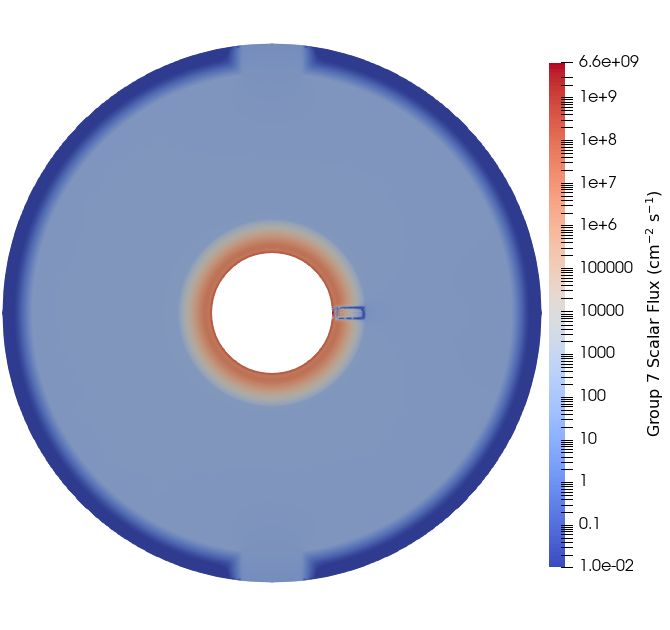
\includegraphics[width=\textwidth]{images/demos/bwr_shield/neutron_field/group_7.png}
        \caption{Group 7 neutron flux ($5.80\times 10^{-2}\text{ eV } \leq E < 1.40\times 10^{-1}\text{ eV}$).}
        \label{fig:demo:bwr:neutron:g7}
    \end{subfigure}
    \caption{Scalar neutron fluxes for various energy groups in the containment system using the \acrshort{sn} solver.}
    \label{fig:demo:bwr:neutron}
\end{figure}

The streaming penetration in the biological shield allows for the direct illumination of the right side of the containment system by fast neutrons in the second energy group. The scalar fluxes caused by this streaming pathway are approximately two orders of magnitude larger than the scalar fluxes at the interface between the biological shield and containment volume. This then results in an even illumination of the containment system by thermal neutrons in the lower energy groups after several scattering events. There are some deficiencies with these results, notably the presence of oscillations in the numerical solutions near the streaming path and within the concrete biological shield and containment walls. In some locations, these are severe enough to result in negative values of scalar fluxes, indicated by the minimum of the logarithmic scale being set to $10^{-2}$. This is due to an under refined mesh in these regions as neutrons attenuate quite rapidly along any direction in concrete due to the effects of down-scattering and absorption. Some ray effects can also be seen in Figure~\ref{fig:demo:bwr:neutron:g2}, indicating that additional angular directions may be required to resolve this deep penetration.

The neutronics model presented above was then coupled to the \acrshort{fvm} mobile depletion solver and the incompressible finite volume fluids solver in the \acrshort{moose} \texttt{NavierStokes} module with the coupling approach outlined in Section~\ref{solver:implementation:coupling}. This was used to model the formation and transport of $\mathrm{^{41}Ar}$ over the air subdomain of the containment structure. Both the fluids simulation and the mobile depletion simulation used first order upwinding. The fluids simulation used the properties of air at $\mathrm{20\text{ }^{\circ}C}$ and atmospheric pressure. An inflow boundary condition was applied to the northern containment airlock with a fixed velocity of $v = \{0.0, -100.0\}$ (cm s\textsuperscript{-1}), and initial conditions are zero velocity and zero pressure. The southern airlock had an outflow boundary condition applied which enforced a fixed pressure boundary condition of $0$ (Pa\textsubscript{g}). The remaining wall boundaries used no-slip boundary conditions. Turbulence modelling was handled using a simple mixing length model on all containment surfaces. This choice of a turbulence model is largely inappropriate for large volume systems such as this containment structure, it was motivated by the limited number of turbulence models supported in the open-source capabilities of the \texttt{NavierStokes} module at the time of performing this work. The value of $Sc_{t}$ chosen for this case is $0.7$ \cite{turbulent_schmidt_numbers}. The fluid mesh is different than that of the neutronics mesh owing to the need to resolve boundary layers when solving for the underlying flow field. The mesh was generated in Coreform Cubit with 99,400 quadrilateral elements, which is shown in Figure~\ref{fig:demo:bwr:flow_mesh}. 

\begin{figure}[H]
    \centering
    \begin{subfigure}[b]{0.495\textwidth}
        \centering
        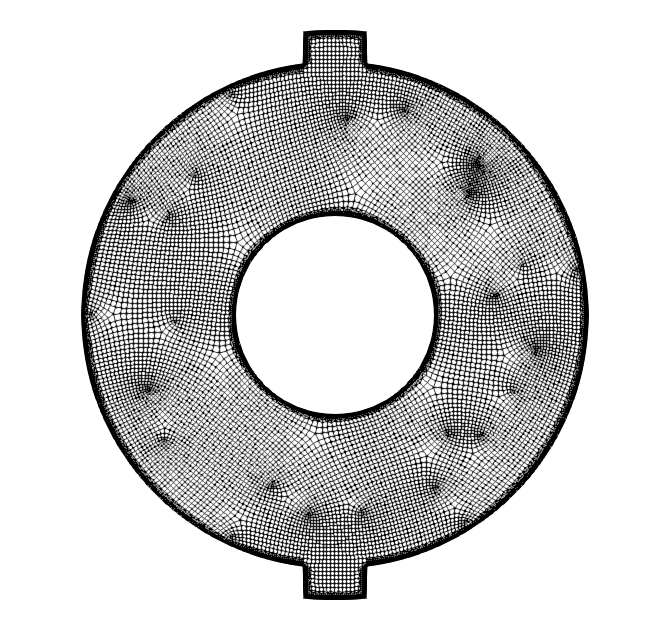
\includegraphics[width=\textwidth]{images/demos/bwr_shield/flow_mesh.png}
        \caption{Full mesh.}
        \label{fig:demo:bwr:mesh:flow_full}
    \end{subfigure}
    \hfill
    \begin{subfigure}[b]{0.495\textwidth}
        \centering
        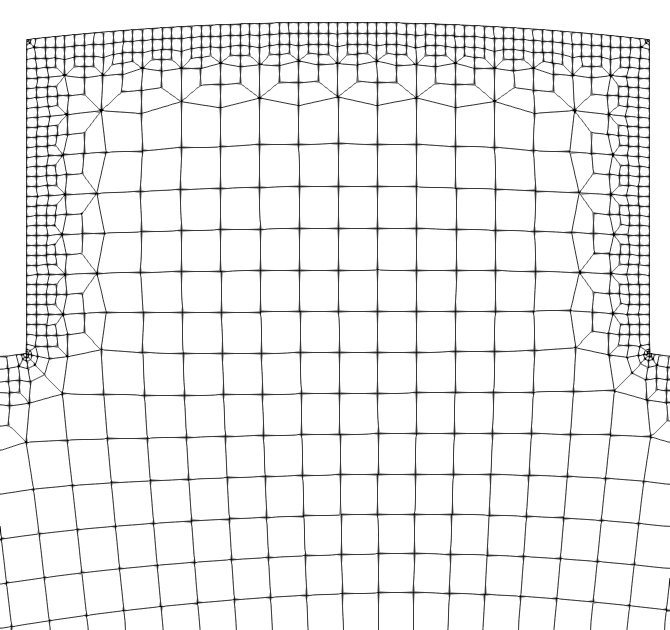
\includegraphics[width=\textwidth]{images/demos/bwr_shield/flow_mesh_close.png}
        \caption{Mesh refinement near the inlet boundary.}
        \label{fig:demo:bwr:mesh:flow_bnd}
    \end{subfigure}
    \caption{Mesh used for the 2D flow and mobile depletion calculations in a containment system.}
    \label{fig:demo:bwr:flow_mesh}
\end{figure}

The mobile depletion model used microscopic transmutation cross sections generated by \texttt{OpenMC} in the same manner as the macroscopic cross sections used for the radiation transport solve. An inflow boundary condition is applied on the northern containment airlock for the mobile depletion equations using the number densities of the nuclide constituents of air at $\mathrm{20\text{ }^{\circ}C}$ and atmospheric pressure. The initial conditions for the mobile depletion calculation are the same as that of the inflow boundary. A time step of $\mathrm{0.5}$ s was used to resolve the flow field and nuclide distributions simultaneously with a total simulation time of 300~s. The Newton solver was used with an absolute tolerance of $10^{-8}$ and a relative tolerance of $10^{-8}$. The Newton solver was chosen because the small size of the system of equations allows for the formation of the Jacaobian matrix for preconditioning without a large memory penalty. The neutron transport calculation was projected onto the mobile depletion mesh using a \texttt{MultiAppGeneralFieldShapeEvaluationTransfer}, which conserves the integral of the scalar fluxes over the entire domain. The results for the velocity fields within the containment system can be found in Figure~\ref{fig:demo:bwr:vel}. The $\mathrm{^{41}Ar}$ activity distribution within the containment system can be found in Figure~\ref{fig:demo:bwr:ar41}, where the activity $\Lambda_{i}(\vec{r}, t)$ is defined as:
\begin{equation}
    \Lambda_{i}(\vec{r}, t) = \lambda_{i}N_{i}(\vec{r}, t)\text{.}
\end{equation}

\begin{figure}[H]
    \centering
    \begin{subfigure}[b]{0.495\textwidth}
        \centering
        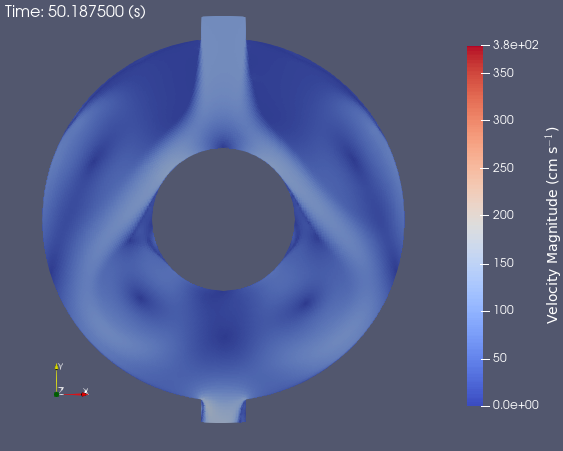
\includegraphics[width=\textwidth]{images/demos/bwr_shield/vel/vel_50s.png}
        \caption{$t = 50$ s.}
        \label{fig:demo:bwr:vel:50s}
    \end{subfigure}
    \hfill
    \begin{subfigure}[b]{0.495\textwidth}
        \centering
        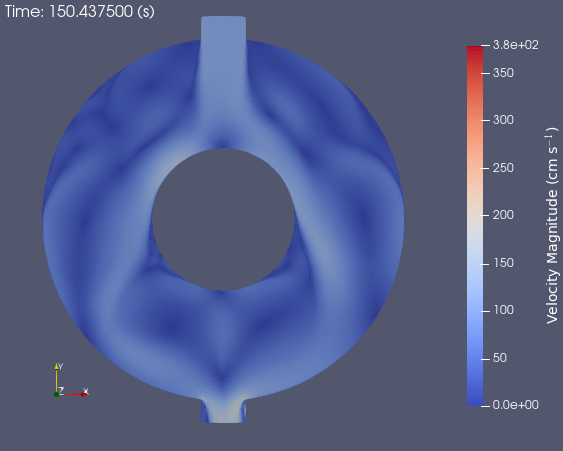
\includegraphics[width=\textwidth]{images/demos/bwr_shield/vel/vel_150s.png}
        \caption{$t = 150$ s.}
        \label{fig:demo:bwr:vel:150s}
    \end{subfigure}
    \hfill
    \begin{subfigure}[b]{0.495\textwidth}
        \centering
        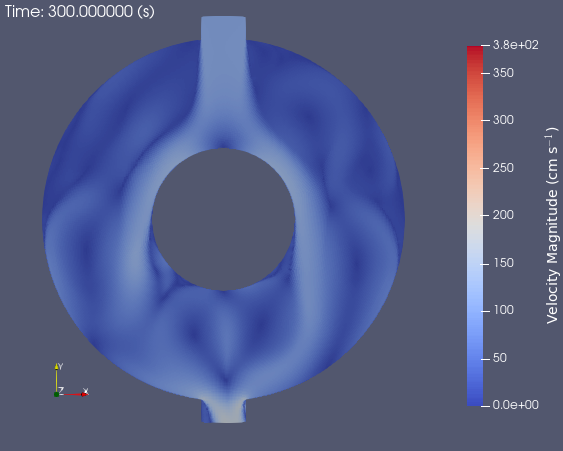
\includegraphics[width=\textwidth]{images/demos/bwr_shield/vel/vel_300s.png}
        \caption{$t = 300$ s.}
        \label{fig:demo:bwr:vel:300}
    \end{subfigure}
    \caption{Velocity profile in the containment system at different points in time.}
    \label{fig:demo:bwr:vel}
\end{figure}

Several interesting features can be noted in Figure~\ref{fig:demo:bwr:ar41}. The first is that $\mathrm{^{41}Ar}$ preferentially forms on the right side of the containment system as opposed to the left. This is due to the deep penetration in the biological shield, resulting in a skew in the scalar flux distributions within containment. The flow field within containment forms large eddies and vortices behind the large obstruction posed by the reactor and biological shield. $\mathrm{^{41}Ar}$ is than entrapped in these eddies, forming areas of high activity relative to other regions of the containment volume. Finally, at the beginning of the simulation $\mathrm{^{41}Ar}$ is preferentially collected in the left-hand side of the outgoing containment airlock. This is due to scattered fast neutrons from the bioshield penetration, which can be seen in Figure~\ref{fig:demo:bwr:neutron:g2} where they illuminate the left-hand side of the containment airlock. 

\begin{figure}[H]
    \centering
    \begin{subfigure}[b]{0.495\textwidth}
        \centering
        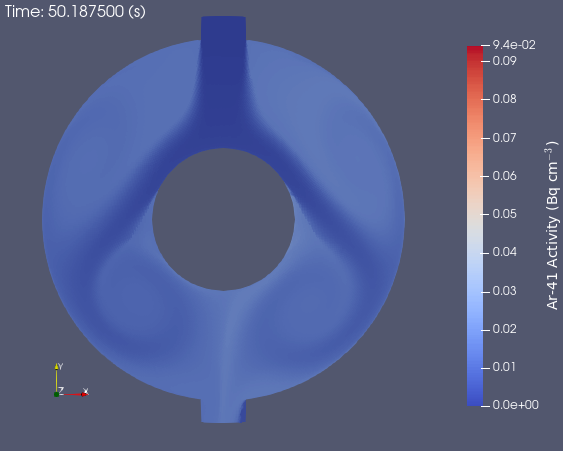
\includegraphics[width=\textwidth]{images/demos/bwr_shield/ar41/ar41_50s.png}
        \caption{$t = 50$ s.}
        \label{fig:demo:bwr:ar41:50s}
    \end{subfigure}
    \hfill
    \begin{subfigure}[b]{0.495\textwidth}
        \centering
        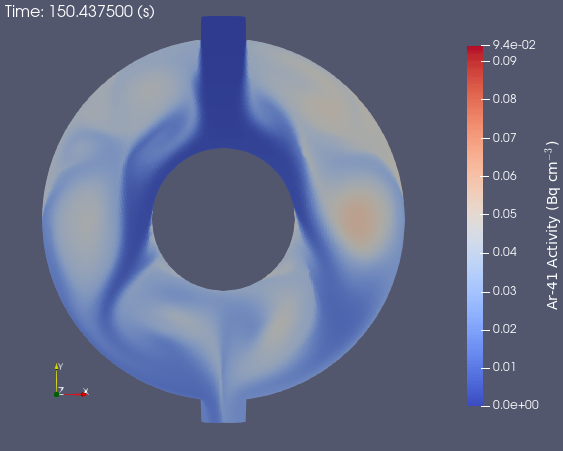
\includegraphics[width=\textwidth]{images/demos/bwr_shield/ar41/ar41_150s.png}
        \caption{$t = 150$ s.}
        \label{fig:demo:bwr:ar41:150s}
    \end{subfigure}
    \hfill
    \begin{subfigure}[b]{0.495\textwidth}
        \centering
        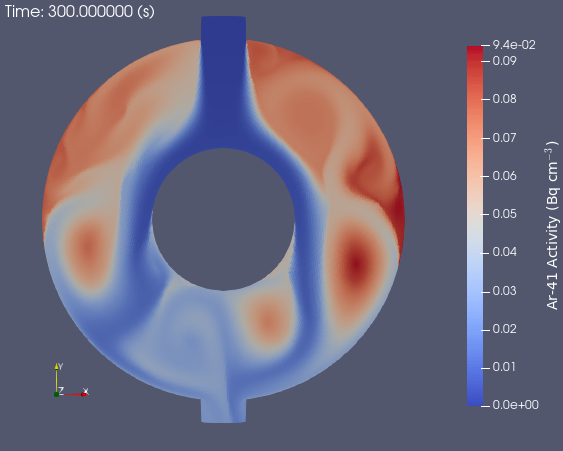
\includegraphics[width=\textwidth]{images/demos/bwr_shield/ar41/ar41_300s.png}
        \caption{$t = 300$ s.}
        \label{fig:demo:bwr:ar41:300}
    \end{subfigure}
    \caption{$\mathrm{^{41}Ar}$ distribution in the containment system at different points in time.}
    \label{fig:demo:bwr:ar41}
\end{figure}

\section{Cs-137 Release Plume Dose Rate Modelling}
\label{demos:demonstrations:cs_137_plume}

The second demonstration problem evaluates the radiation field caused by a $\mathrm{^{137}Cs}$ release from a containment structure using a representative model in 2D. This system consists of a 75~m tall containment structure with a 60~m tall stack attached on the left. The outlet of this stack is 2.08~m wide. The containment system and stack are immersed in a 850~m long and 150~m tall domain which acts as a surrogate domain for the local weather system. The geometry of this problem can be found in Figure~\ref{fig:demo:plume:geo:full}. $\mathrm{^{137}Cs}$ undergoes two decays before a characteristic gamma photon is released at 662~keV:
\begin{equation*}
    \mathrm{^{137}Cs} \xrightarrow{\mathrm{\beta-}} \mathrm{^{137m}Ba} \xrightarrow{\mathrm{\gamma}} \mathrm{^{137}Ba}\text{,}
\end{equation*}
which lags the formation of the photon source for the plume.

\begin{figure}[H]
    \centering
    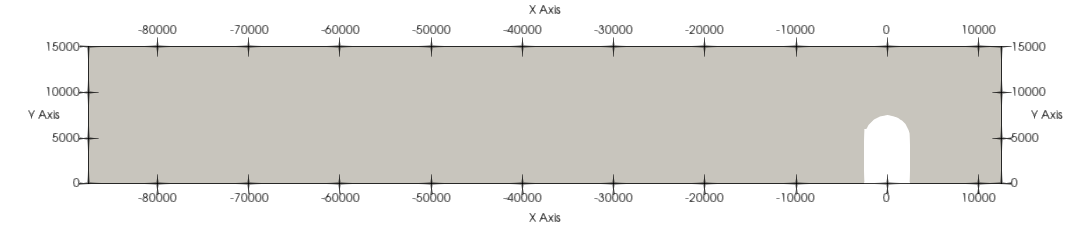
\includegraphics[width=\textwidth]{images/demos/plume/domain.png}
    \caption{2D domain for dispersion and photon transport. All units are in cm.}
    \label{fig:demo:plume:geo:full}
\end{figure}

Plume transport and decay is modelled using the \acrshort{fvm} mobile depletion solver and the incompressible finite volume fluids solver in the \texttt{NavierStokes} module, where the coupling approach presented in Figure~\ref{fig:solver:1_way_photon_neutron} is adopted. Both the fluids simulation and the mobile depletion calculation used first order upwinding. The fluid properties used are that of air at $20\text{ }^{\circ}\text{C}$ and atmospheric pressure. An inflow boundary condition is placed on the right side of the domain with an inflow velocity of $\vec{v} = \{-100.0, 0.0\}$ cm s\textsuperscript{-1} and a second inflow boundary condition is placed at the outlet of the stack with an inflow velocity of $\vec{v} = \{0.0, 100.0\}$ cm s\textsuperscript{-1}. The ground and body of the containment structure used no-slip boundary conditions while the top of the domain used a slip boundary condition. The left side of the domain enforced a zero pressure outflow boundary. Similar to the previous demonstration problem, turbulence modelling was accomplished with a mixing length turbulence model, which was applied to the same surfaces as the no-slip boundary conditions. This choice is largely inappropriate for modelling turbulence in an atmospheric transport setting, and is once again motivated by the lack of native options for turbulence modelling in \acrshort{moose}. The value of $Sc_{t}$ chosen for this case was $0.7$, which is the default reported by literature for trace species transport in atmospheric settings when representative experiments have not been performed \cite{turbulent_schmidt_numbers}. The mobile depletion solver applied an inflow boundary condition on the stack for the $\mathrm{^{137}Cs}$ number density which corresponded to an activity of 1~MBq. The problem domain was meshed in Coreform Cubit with 49,803 quadrilateral elements. The section of this mesh which corresponds to the region near the containment system can be found below in Figure~\ref{fig:demo:plume:flow:mesh}.
\begin{figure}[H]
    \centering
    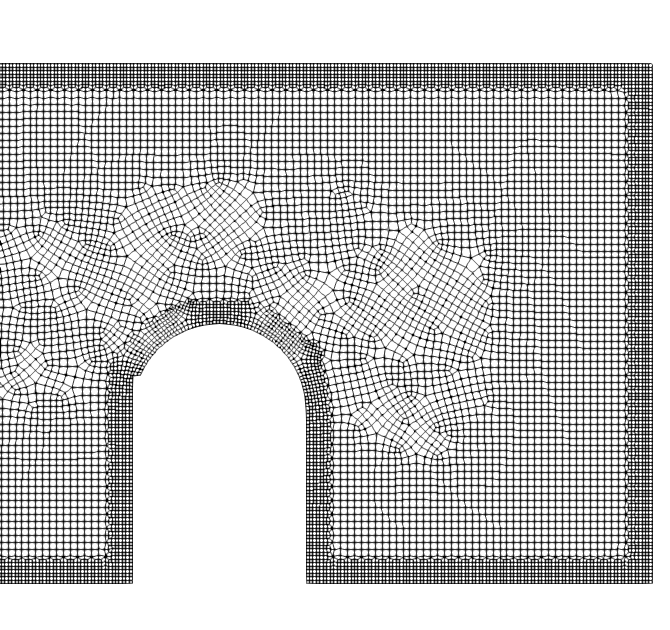
\includegraphics[width=0.6\textwidth]{images/demos/plume/flow_mesh.png}
    \caption{Mesh used for the plume mobile depletion and flow model.}
    \label{fig:demo:plume:flow:mesh}
\end{figure}
\noindent The Newton solver provided by \acrshort{moose} was used with a relative convergence criteria of $10^{-8}$ based on an initial residual vector magnitude of $1.011341\times 10^{1}$. Further reductions to the relative convergence criteria did not modify the flow profile around the containment system in the first minute of simulation time. The simulation was time stepped over a period of 10 minutes using a $\Delta t$ of 5~s. The resulting $\mathrm{^{137}Cs}$ number density distribution can be found in Figure~\ref{fig:demo:plume:flow:cs}.
\begin{figure}[H]
    \centering
    \begin{subfigure}[b]{0.68\textwidth}
        \centering
        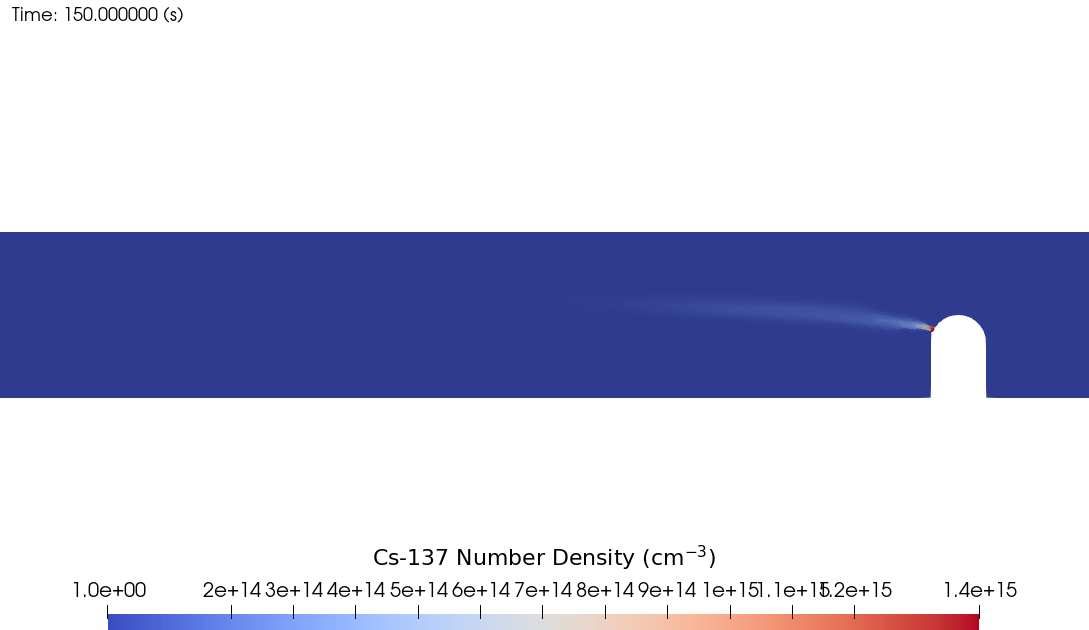
\includegraphics[width=\textwidth]{images/demos/plume/cs/cs137_150s.png}
        \caption{$t = 150$ s.}
        \label{fig:demo:plume:flow:cs:150}
    \end{subfigure}
    \hfill
    \begin{subfigure}[b]{0.68\textwidth}
        \centering
        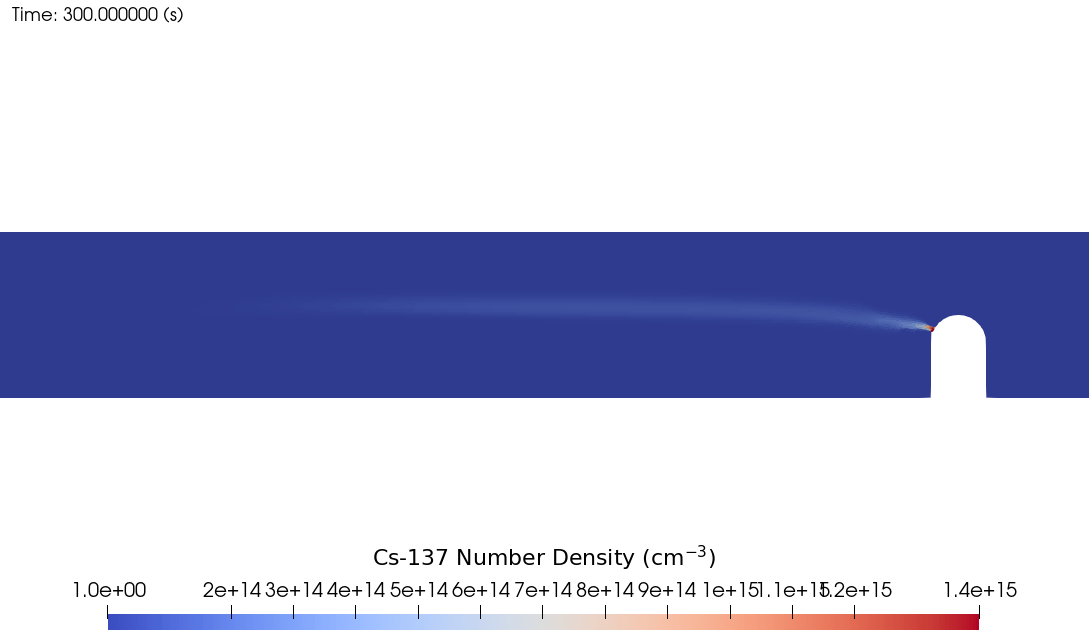
\includegraphics[width=\textwidth]{images/demos/plume/cs/cs137_300s.png}
        \caption{$t = 300$ s.}
        \label{fig:demo:plume:flow:cs:300}
    \end{subfigure}
    \hfill
    \begin{subfigure}[b]{0.68\textwidth}
        \centering
        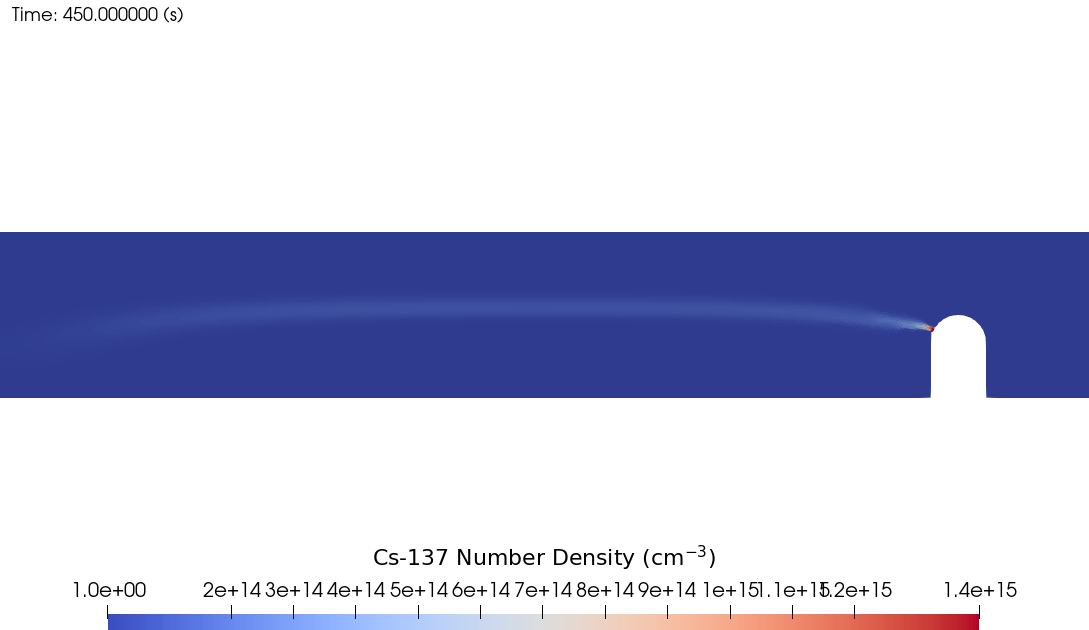
\includegraphics[width=\textwidth]{images/demos/plume/cs/cs137_450s.png}
        \caption{$t = 450$ s.}
        \label{fig:demo:plume:flow:cs:450}
    \end{subfigure}
    \caption{$\mathrm{^{137}Cs}$ dispersion in the wake of a containment system.}
    \label{fig:demo:plume:flow:cs}
\end{figure}

\begin{figure}[H]
    \centering
    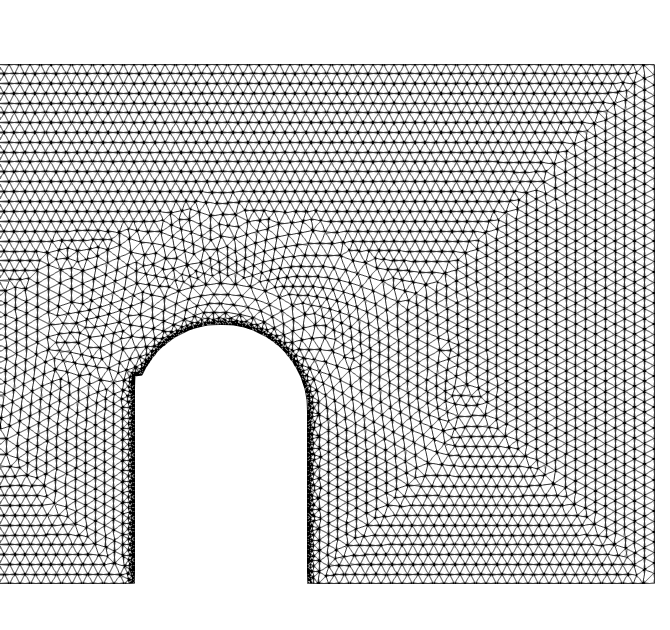
\includegraphics[width=0.6\textwidth]{images/demos/plume/rad_mesh.png}
    \caption{Section of the mesh used for the plume photon transport model.}
    \label{fig:demo:plume:rad:mesh}
\end{figure}

The modelling of the radiation fields which corresponded with the plume in Figure~\ref{fig:demo:plume:flow:cs} was performed with the \acrshort{sn} transport solver. Point-wise isotropic scattering photon cross sections at 662~keV were used from Shultis and Faw \cite{radiation_shielding} as \texttt{OpenMC} is not capable of computing multi-group photon cross sections at present time. All boundaries in the radiation transport model used vacuum boundary conditions. The problem domain was generated with Coreform Cubit using 34,250 triangular elements; a section of this mesh can be found below in Figure~\ref{fig:demo:plume:rad:mesh}. A Gauss-Chebyshev product quadrature with 10 polar angles and 10 azimuthal angles, resulting in a total of 400 angular unknowns. This problem used the \acrshort{pjfnk} solver with block Jacobi preconditioning and 600 \acrshort{gmres} vectors. A relative convergence criteria of $10^{-8}$ was used based on the initial residual vector magnitude of $2.220910\times 10^{1}$ which was obtained for the first timestep. Photon transport was time stepped in lock-step with the mobile depletion calculation in accordance with the coupling strategy discussed in Section~\ref{solver:implementation:coupling}. The resulting 662~keV photon fields from this coupled problem can be found in Figure~\ref{fig:demo:plume:rad:photon}.

\begin{figure}[H]
    \centering
    \begin{subfigure}[b]{0.68\textwidth}
        \centering
        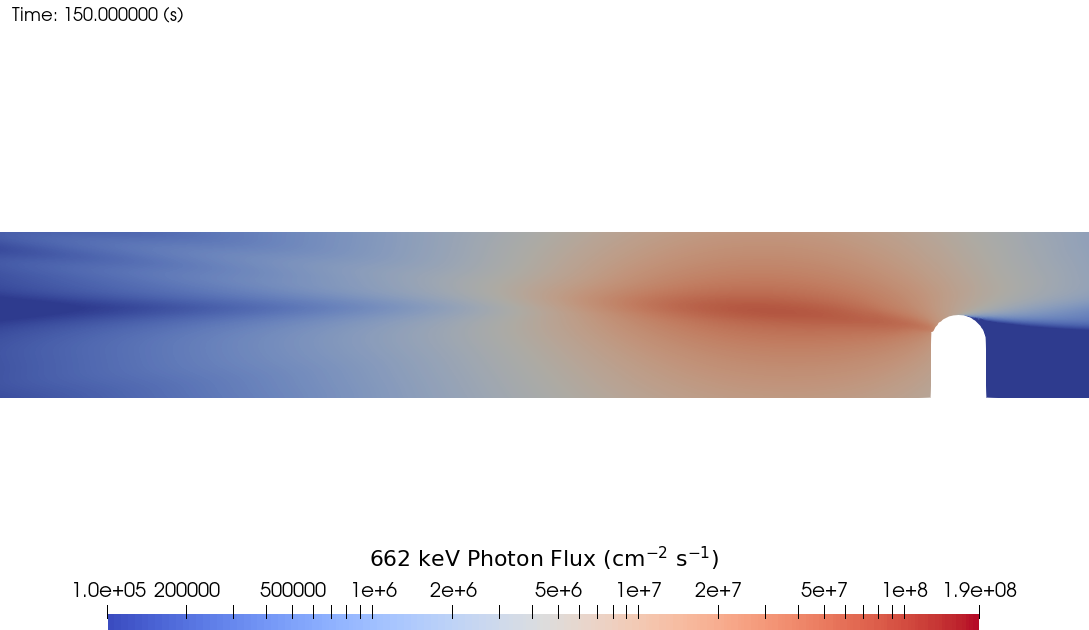
\includegraphics[width=\textwidth]{images/demos/plume/photon/flux_log_150s.png}
        \caption{$t = 150$ s.}
        \label{fig:demo:plume:rad:photon:150}
    \end{subfigure}
    \hfill
    \begin{subfigure}[b]{0.68\textwidth}
        \centering
        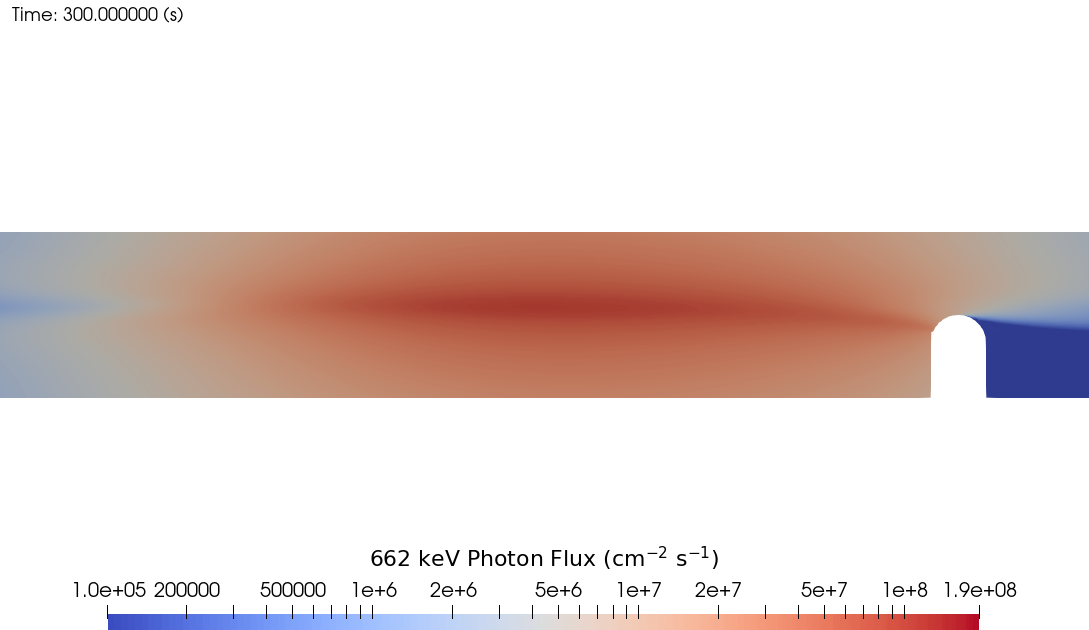
\includegraphics[width=\textwidth]{images/demos/plume/photon/flux_log_300s.png}
        \caption{$t = 300$ s.}
        \label{fig:demo:plume:rad:photon:300}
    \end{subfigure}
    \hfill
    \begin{subfigure}[b]{0.68\textwidth}
        \centering
        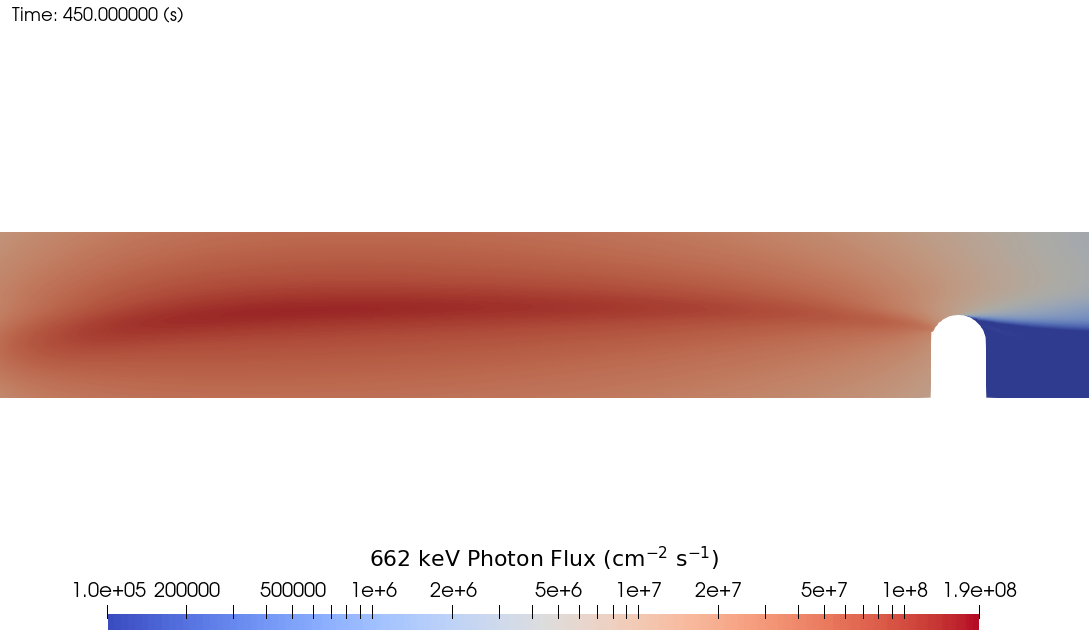
\includegraphics[width=\textwidth]{images/demos/plume/photon/flux_log_450s.png}
        \caption{$t = 450$ s.}
        \label{fig:demo:plume:rad:photon:450}
    \end{subfigure}
    \caption{662 keV photon fields from the $\mathrm{^{137}Cs}$ plume in Figure~\ref{fig:demo:plume:flow:cs}.}
    \label{fig:demo:plume:rad:photon}
\end{figure}

As expected, the 662~keV photon flux lags behind the front of the plume due to the time required for the double decay from $\mathrm{^{137}Cs}$ to $\mathrm{^{137}Ba}$. Every time step in Figure~\ref{fig:demo:plume:rad:photon} shows how the containment structure shields the area to its right from the vast majority of the photon flux. However, after multiple scattering events, some photons reach the region in the shadow of the containment structure, showcasing the importance of radiation scattering. This effect is difficult to simulate with lower fidelity methods such as the point kernel method with buildup factors \cite{radiation_shielding}. Some numerical errors can be seen in the photon scalar flux distribution; the first being ray effects to the left of the front of the plume. These persist across the first two time steps until the photon source is evenly distributed across the majority of the plume. The second numerical artifact is a small region near the top of the containment structure which generated a negative value of the scalar photon flux. As with the numerical oscillations in the neutron fluxes in Section~\ref{demos:demonstrations:ar41_bwr} this is caused by an under refined mesh near the top of the containment structure where there is a series of elements that have line of sight with both a vacuum boundary condition and the plume. This results in a strong heterogeneity within the numerical solution, which is difficult for the \acrshort{saaf} approach to resolve. 